% !TEX program = xelatex
\documentclass[12pt,a4paper]{article}

% بسته‌های ضروری
\usepackage{amsmath, amssymb}
\usepackage{graphicx} % برای قرار دادن لوگو
\graphicspath{{Pictures/}} % مسیر پوشه عکس‌ها
\usepackage[left=2.5cm,right=2.5cm,top=3cm,bottom=3cm]{geometry}
\usepackage[colorlinks=true,linkcolor=blue,citecolor=blue]{hyperref}
\usepackage{xepersian}

% تنظیمات فونت
\settextfont[Scale=1]{B Yas}
\setlatintextfont[Scale=1]{Times New Roman}
\setdigitfont[Scale=1]{B Yas}
\defpersianfont\nastaliqsmall[Scale=1.2]{IranNastaliq}

\renewcommand\baselinestretch{1.5}
% رفع مشکل نمایش بولت‌پوینت‌ها در زی‌پرشین
\renewcommand{\labelitemi}{$\bullet$}

\begin{document}

% --- صفحه عنوان ---
\thispagestyle{empty}
\vspace*{-1.5cm}

\begin{figure}[ht]
\centering
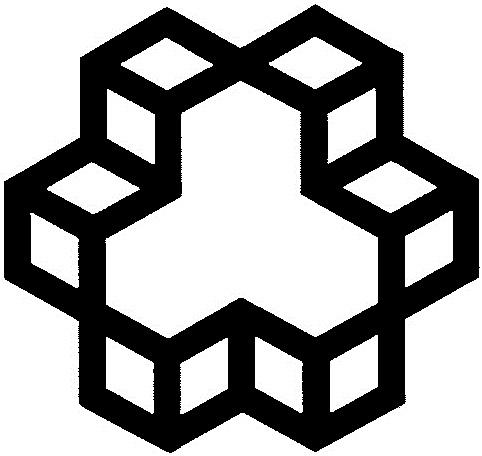
\includegraphics[width=2.5cm]{kntuarm}
\end{figure}
\vspace{-0.5cm}

\begin{center}
{\nastaliqsmall دانشگاه صنعتی خواجه نصیرالدین طوسی}\\[0.2cm]
{\nastaliqsmall دانشکده مهندسی کامپیوتر}\vspace{1.5cm}\\
{\LARGE پیشنهاد پروژه پایانی کارشناسی}\vspace{1.5cm}\\
{\large عنوان:}\vspace{4mm}\\
{\huge\textbf{تحلیل ساختارهای احتمالی در گراف اسپنرها و بررسی توابع توزیع بهینه}}\vspace{1.5cm}\\
{\large نویسنده:}\vspace{4mm}\\
{\Large\textbf{محمدرضا احمدی}}\vspace{1.5cm}\\
{\large استاد راهنما:}\vspace{4mm}\\
{\Large\textbf{دکتر حسین جوهری}}\vspace{1.5cm}\\
{\large تابستان ۱۴۰۵}
\end{center}

% --- فهرست مطالب ---
\newpage
\tableofcontents

% --- شروع متن اصلی ---
\newpage
\pagenumbering{arabic}

\section{مقدمه}
با فرض یک گراف $G$، یک گراف اسپنر (\lr{Graph Spanner}) یا به سادگی اسپنر، زیرگرافی از $G$ است که طول کوتاه‌ترین مسیرها در آن را تا حد مشخصی از خطا یا اعوجاج (\lr{Distortion}) حفظ می‌کند. این خطا معمولاً به صورت ضربی (\lr{Multiplicative})، جمعی (\lr{Additive}) یا ترکیبی از هر دو تعریف می‌شود. مفهوم اسپنرها برای نخستین بار توسط پلگ (\lr{Peleg}) و شافر (\lr{Schäffer}) معرفی گردید. امروزه محاسبه و یافتن اسپنرهای خلوت (\lr{Sparse}) یا کم‌وزن، کاربردهای تئوریک و عملی گسترده‌ای در مسائل گوناگون طراحی شبکه دارد که از میان آن‌ها می‌توان به فشرده‌سازی گراف، محاسبات توزیع‌شده و شبکه‌های ارتباطی اشاره کرد.

هدف اصلی این پژوهش، تمرکز بر روی مدل‌های احتمالی (\lr{Probabilistic Models}) برای یافتن گراف اسپنرها است. در این راستا، قصد داریم با مطالعه عمیق این مدل‌ها، چالش‌ها و ساختارهای تئوریک این حوزه را بررسی کرده و گامی در جهت تحلیل توابع توزیع بهینه در گراف‌ها برداریم.

\section{تعاریف و مفاهیم اولیه}
با فرض یک گراف $G$ که ممکن است دارای وزن روی یال‌ها باشد، یک گراف اسپنر (\lr{Graph Spanner}) یا به اختصار اسپنر، زیرگرافی مانند $G'$ است که طول کوتاه‌ترین مسیرها در $G$ را تا حد مشخصی از خطا یا اعوجاج (\lr{Distortion}) (به عنوان مثال، خطای جمعی و/یا ضربی) حفظ می‌کند \cite{survey}. 

تعاریف و فرمول‌بندی‌های مختلفی برای گراف اسپنرها وجود دارد. بیشتر اسپنرها را می‌توان با استفاده از دو پارامتر مشخص کرد: یک تابع اعوجاج $f$ که مشخص می‌کند فواصل گراف اصلی تا چه حد مجاز به تغییر و اعوجاج هستند، و یک زیرمجموعه $P \subseteq V \times V$ که زوج‌رئوسی از گراف اولیه را تعیین می‌کند که فواصل آن‌ها باید به طور تقریبی حفظ شود. به عبارت دیگر، زیرگراف $G' = (V', E')$ یک اسپنر با اعوجاج $f$ برای $P \subseteq V \times V$ است، اگر رابطه زیر برقرار باشد \cite{survey}:
$$d_{G'}(u, v) \le f(d_G(u, v))$$
برای تمام $(u, v) \in P$. شایان ذکر است که برای هر زیرگراف $G'$ از $G$ همواره داریم $d_G(u, v) \le d_{G'}(u, v)$؛ از این رو، شرط می‌کنیم که تابع اعوجاج در نامساوی $f(x) \ge x$ صدق کند \cite{survey}.

\vspace{0.4cm}
\noindent دو مورد از رایج‌ترین انواع تابع اعوجاج $f$ که ما در این پژوهش با آن‌ها سر و کار داریم، به شرح زیر هستند \cite{survey}:
\begin{itemize}
    \item \textbf{اسپنر ضربی (\lr{Multiplicative} یا $t$-اسپنر):} در این حالت، تابع اعوجاج به صورت $f(x) = tx$ برای یک مقدار ثابت $t \ge 1$ تعریف می‌شود. مقدار $t$ به عنوان ضریب کشیدگی (\lr{Stretch Factor}) شناخته می‌شود. این بدان معناست که فواصل در گراف اسپنر، حداکثر با ضریبی از $t$ کشیده می‌شوند. برخی از نویسندگان به جای $t$ از متغیر $k$ برای نشان دادن ضریب کشیدگی استفاده می‌کنند.
    \item \textbf{اسپنر جمعی (\lr{Additive}):} در این نوع، تابع اعوجاج به صورت $f(x) = x + \beta$ تعریف می‌گردد. به عبارت دیگر، فواصل در اسپنرهای جمعی بیشتر از $\beta$ واحد (یا یال) طولانی‌تر نمی‌شوند. این زیرگراف‌ها فواصل طولانی را با نسبتی نزدیک به ۱ حفظ می‌کنند. اسپنرهای جمعی گاهی اوقات $+\beta$-اسپنر نیز نامیده می‌شوند.
\end{itemize}

بیشتر مسائل اسپنر را می‌توان از طریق پارامترهای اعوجاج $(\alpha, \beta)$ و زوج‌رئوس $P$ که فواصلشان باید حفظ شود، مشخص کرد. برای خلاصه‌سازی نمادگذاری، معمولاً از عبارت $(\alpha, \beta, P)$-اسپنر، و یا برای اعوجاج‌های کلی از $(f, P)$-اسپنر استفاده می‌کنیم. همچنین باید توجه داشت که اگرچه تمام انواع اسپنرها برای گراف‌های وزن‌دار و بدون وزن خوش‌تعریف هستند، اما بررسی اسپنرهای جمعی در زمانی که گراف بدون وزن باشد، طبیعی‌تر است. در واقع، اگر گراف $G$ دارای وزن‌های یال به طور دلخواه بزرگ باشد، ممکن است مقدار $\beta$ ای وجود داشته باشد که هیچ $\beta$-اسپنر جمعی به جز خود گراف $G$ برای آن یافت نشود \cite{survey}.

\subsection{پیچیدگی محاسباتی مسئله}
برای درک بهتر دشواری این مسئله، رهیافت جستجوی جامع (\lr{Brute Force}) برای یافتن یک اسپنر بهینه (با کمترین تعداد یال) را در نظر بگیرید. روند این الگوریتم به شرح زیر است:
\begin{enumerate}
    \item ابتدا طول کوتاه‌ترین مسیر بین تمام زوج‌رئوس در گراف اصلی $G$ محاسبه می‌شود (به عنوان مثال با استفاده از الگوریتم فلوید-وارشال در زمان $O(|V|^3)$).
    \item سپس تمامی زیرگراف‌های ممکن گراف $G$ تولید می‌شوند. از آنجا که گراف دارای $|E|$ یال است، دقیقاً $2^{|E|}$ زیرگراف متمایز وجود دارد.
    \item برای هر یک از این $2^{|E|}$ زیرگراف، الگوریتم یافتن کوتاه‌ترین مسیر مجدداً اجرا شده و بررسی می‌شود که آیا شرط اعوجاج برای تک‌تک زوج‌رئوس برقرار است یا خیر.
\end{enumerate}
محاسبه و بررسی این شروط برای تمام زیرگراف‌ها، زمان اجرای کل این رویکرد بدیهی را به مرتبه نمایی $O(2^{|E|} \cdot |V|^3)$ می‌رساند که حتی برای گراف‌هایی با اندازه متوسط نیز کاملاً غیرقابل اجراست.

با توجه به این انفجار ترکیبیاتی، در این پژوهش بدون ارائه اثبات می‌پذیریم که مسئله یافتن یک گراف اسپنر با کمترین تعداد یال ممکن، در دسته مسائل \textbf{\lr{NP-Hard}} قرار می‌گیرد. همین پیچیدگی محاسباتی و سختی ذاتی مسئله است که استفاده از الگوریتم‌های تقریبی و به ویژه \textbf{مدل‌های احتمالی} (که محوریت این پژوهش را تشکیل می‌دهند) را به تنها راهکارهای عملی و ارزشمند تبدیل می‌کند.

\newpage
\section{اهداف}
برای تشریح دقیق اهداف این پژوهش، مرور روند توسعه مدل‌های احتمالی در گراف اسپنرها ضروری است. میلر (\lr{Miller}) و همکاران اولین الگوریتم تصادفی را برای تولید یک اسپنر با احتمال بالا ارائه کردند \cite{miller}. نتیجه اصلی آن‌ها منجر به تولید یک $O(k)$-اسپنر ضربی با احتمال بالا، با اندازه مورد انتظار $O(n^{1+1/k} \log k)$ و در زمان مورد انتظار $O(m)$ می‌شود \cite{miller}.

الکین (\lr{Elkin}) و نیمان (\lr{Neiman}) با ارائه یک ساختار تصادفی که یک $(2k-1)$-اسپنر با $O(n^{1+1/k}\varepsilon^{-1})$ یال را با احتمال $1-\varepsilon$ محاسبه می‌کند، کار میلر و همکاران را بهبود بخشیدند \cite{elkin}. آن‌ها علاوه بر این، تحلیلی از زمان اجرا و تعداد یال‌ها برای مدل‌های محاسباتی \lr{PRAM} و \lr{CONGEST} ارائه دادند \cite{elkin}.

برای درک بهتر این رویکرد، یادآوری می‌کنیم که با فرض پارامتر $\lambda > 0$، توزیع نمایی (\lr{Exponential Distribution}) توسط تابع چگالی احتمال (\lr{PDF}) زیر تعریف می‌شود \cite{elkin}:
$$
p_\lambda(x) =
\begin{cases}
\lambda e^{-\lambda x} & x \ge 0 \\
0 & x < 0
\end{cases}
$$
ما یک بردار تصادفی $x$ که از این توزیع استخراج شده باشد را با $x \sim Exp(\lambda)$ نشان می‌دهیم \cite{elkin}. 
الگوریتم معرفی شده توسط الکین و نیمان به شکل زیر ساختاریافته است \cite{elkin}:

\vspace{0.5cm}
\noindent\begin{minipage}{\textwidth}
\begin{latin}
\noindent\rule{\textwidth}{0.4pt}
\textbf{Algorithm 6} \textsc{Rand Exp} $(2k - 1)$--\textsc{Spanner}$(G, k, c)$ \\
\rule{\textwidth}{0.4pt}
$\lambda \gets \frac{\ln(cn)}{k}$ \\
\textbf{for} $u \in V$ \textbf{do} \\
\hspace*{1em} Draw $r_u \sim Exp(\lambda)$ \\
\hspace*{1em} $u$ broadcasts $r_u$ to all vertices $v$ within distance $k$ \\
\hspace*{1em} \textbf{if} $x$ receives a message from $u$ \textbf{then} \\
\hspace*{2em} $x$ stores the value $m_u(x) = r_u - d_G(u, x)$ \\
\hspace*{2em} $x$ also stores a neighboring vertex $p_u(x)$ along a shortest path from $u$ to $x$ (if there is more than one possibility, one is selected randomly) \\
\hspace*{1em} \textbf{end if} \\
\textbf{end for} \\
$m(x) \gets \max_{u \in V} m_u(x)$ \\
\textbf{for} $x \in V$ \textbf{do} \\
\hspace*{1em} $E' \gets E' \cup C(x) = \{ (x, p_u(x)) : m_u(x) \ge m(x) - 1 \}$ \\
\textbf{end for} \\
\textbf{return} $E'$ \\
\rule{\textwidth}{0.4pt}
\end{latin}
\end{minipage}
\vspace{0.5cm}

دلیل کلیدی برای استفاده از توزیع نمایی جهت تعیین پیام‌های ارسال‌شده از هر راس، ویژگی بی‌حافظگی (\lr{Memoryless Property}) آن است \cite{elkin}. این بدان معناست که اگر $x \sim Exp(\lambda)$ و $s, t \in \mathbb{R}$، آنگاه $\mathbb{P}(x > s+t \mid x > t) = \mathbb{P}(x > s)$، که نشان می‌دهد این احتمال به مقدار $t$ بستگی ندارد.

با توجه به این پیشینه و ساختار معرفی‌شده، \textbf{هدف اصلی و نهایی این پژوهش}، تمرکز بر روی یکی از دو مسئله باز (\lr{Open Problem}) زیر خواهد بود تا با تحلیل دقیق‌تر مدل‌های احتمالی، گامی در جهت حل یا بهبود آن‌ها برداریم:
\begin{enumerate}
    \item آیا می‌توان ساختار الگوریتم الکین و نیمان را بر روی تابع چگالی احتمال بهینه‌سازی کرد تا تضمین بهتری برای اندازه یک $(2k - 1)$-اسپنر به دست آورد؟
    \item آیا می‌توان یک توزیع احتمالی بر روی یال‌های یک گراف طراحی کرد که نمونه‌برداری تصادفی از آن، با احتمال بالا منجر به تولید یک اسپنر شود؟
\end{enumerate}

\newpage
\begin{thebibliography}{3}
\addcontentsline{toc}{section}{مراجع}
\baselineskip=6mm
\begin{LTRbibitems}
\resetlatinfont
\bibitem{survey}
R. Ahmed, G. Bodwin, F. D. Sahneh, K. Hamm, M. J. L. Jebelli, S. Kobourov, and R. Spence, "Graph Spanners: A Tutorial Review."

\bibitem{miller}
G. L. Miller, R. Peng, A. Vladu, and S. C. Xu, "Improved parallel algorithms for spanners and hopsets," \textit{Proceedings of the 27th ACM Symposium on Parallelism in Algorithms and Architectures}, pp. 192--201, ACM, 2015.

\bibitem{elkin}
M. Elkin and O. Neiman, "Efficient algorithms for constructing very sparse spanners and emulators," \textit{ACM Transactions on Algorithms (TALG)}, vol. 15, no. 1, pp. 1--29, 2018.
\end{LTRbibitems}
\end{thebibliography}

\end{document}